\documentclass{article}
\usepackage[T1]{fontenc}
\usepackage{lmodern}
\usepackage{graphicx}
\usepackage{amsmath,amssymb}
\usepackage[a4paper,margin=2cm]{geometry}
\usepackage[absolute,overlay]{textpos}
\setlength{\TPHorizModule}{1mm}
\setlength{\TPVertModule}{1mm}
\usepackage[indonesian]{babel}
\usepackage{hyperref}
\setlength{\emergencystretch}{2em}
% unit: Halaman 15

\begin{document}

% === Halaman 15 (llm) ===

\vspace{47.52mm}

$p = 2 \rightarrow GF(2):$
\vspace{40mm}
$p = 3 \rightarrow GF(3):$

\vspace{65.34mm}

% deskripsi: Tabel penjumlahan dan perkalian untuk field Galois GF(2)
% bbox normalisasi: [0.2100, 0.2300, 0.6900, 0.3900]
\begin{textblock*}{100.80mm}(44.10mm,68.31mm)
\noindent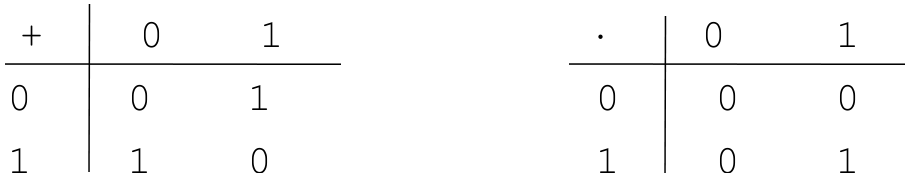
\includegraphics[width=100.80mm,height=47.52mm]{../../images/llm/page_015_img_01.png}%
\end{textblock*}

% deskripsi: Tabel penjumlahan dan perkalian untuk field Galois GF(3)
% bbox normalisasi: [0.2100, 0.5300, 0.7200, 0.7500]
\begin{textblock*}{107.10mm}(44.10mm,157.41mm)
\noindent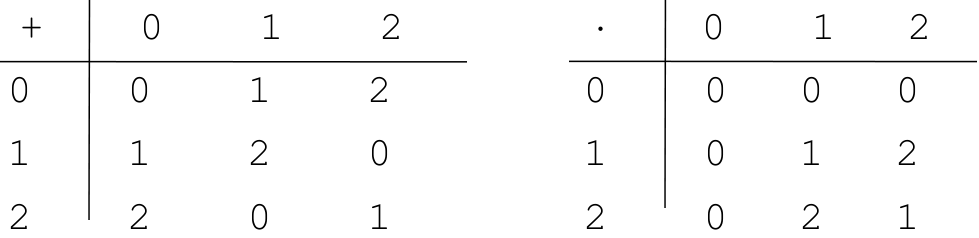
\includegraphics[width=107.10mm,height=65.34mm]{../../images/llm/page_015_img_02.png}%
\end{textblock*}

\end{document}
